The primitive $\OTK$ is intended to decrypt the results of homomorphically evaluated functions (HEFs) that involve arithmetic operations, including comparisons such as equalities and inequalities. For example, in scenarios such as determining whether someone is under 18 years of age or comparing the country of residence with each European Union (EU) member state, since EU addresses usually do not explicitly contain ``EU''or any distinguishing indicator, homomorphic comparisons (HC) pose a significant challenge. Bit-wise Homomorphic Encryption (HE) schemes, such as FHEW and TFHE, offer the fastest HC, with comparisons for two n-bit integers done in $\approx170.n$ microseconds\cite{chillottiFasterPackedHomomorphic2017,chillottiTFHEFastFully2020}.

However, when working with word-based encryption schemes (e.g., BGV, BFV, CKKS), HC performance is not as favourable. Efforts have been made to efficiently implement equality ($EQ_S$) and inequality ($LT_S$) operations within these encryption frameworks. 
\begin{align*}
    &LT_S(a,b) = 
    \begin{cases}
      1, & \text{if } a < b; \\
      0, & \text{if } a \ge b, \\
    \end{cases}   
    &&EQ_S(a,b) = 
    \begin{cases}
      1, & \text{if } a = b; \\
      0, & \text{if } a \neq b. \\
    \end{cases}
  \end{align*}
The implementation of the equality function is straightforward using Fermat's Little Theorem to implement the 
\begin{equation}\label{eq:iszero}
    \mathrm{IsZero}(a-b)=EQ_S(a,b)= 1 - (a-b)^{q-1} \bmod q
\end{equation}
function, often used in practice, although its usage can be challenging due to its sequential multiplications, particularly with large modulus values ($q$).

Kim et al. \cite{kimEfficiencyFHEbasedPrivate2016} introduced an optimization technique. When $a,b \in S=\F_{q^d}$ and $d>1$, they use the multiplicative deep-free Frobenius automorphism operation $x \mapsto x^{q}$. This operation reduces the depth of the equality circuit $EQ(a,b) = 1 - (a-b)^{q^{d}-1}$ from $\ceil{d\log_2(q)}$ to $\ceil{\log_2(d)} + \ceil{\log_2(q-1)}$.

Iliashenko and Zucca~\cite{iliashenkoFasterHomomorphicComparison2021} follow the bit comparison strategy, but instead of bits they split the message into digits that they encode in different slots of plaintext. They use a univariate polynomial to interpolate a function that calculates the sign of the difference between two values
Tan et al.~\cite{tanEfficientPrivateComparison2020} went a bit further by embedding each plaintext in a ciphertext slot, encoding different digits of the plaintext into subfields of $\F_{q^d}$ in each slot. They compared each digit and processed the results using a lexicographic circuit.

One common optimization technique is to use SIMD techniques from certain homomorphic schemes such as BGV and BFV. This involves batching several plaintexts into a single ciphertext, allowing multiple comparisons to be performed simultaneously, which is advantageous when dealing with multiple comparisons over a dataset. Both Tan et al. and Iliashenko and Zucca's solutions use this technique to amortize the cost of each individual comparison.

However, in the ``Anonymous Credentials'' use case, only a single comparison is needed to decide access to an information service, and the values to compare often result from previous calculations involving additions and multiplications, which do not align with the digit decomposition in the proposed encoding. Without digit decomposition, a single comparison of a 15-bit number takes significantly longer ($\sim~4~m~38~s$) with the Iliashenko and Zucca solution compared to the proposed solution ($10s$).








\subsection{Private Set Membership}\label{sec:psm}
Our approach also takes advantage of the \ac{SIMD}, but we aim to optimize a single comparison rather than amortizing the cost over several comparisons. Our comparison primitive is called ``Private Set Membership" (PSM). The $\PSM$ primitive takes an encrypted value $x$ and a set of values $S$ and returns an encryption of 1 if $x\in S$ and an encryption of 0 otherwise.
\begin{equation} \label{eq:psm}
\begin{split}
\PSM: &\intring_q^2,\intring_q^r \rightarrow \intring_q^2\\
      &(\enc{x},\pv{s}) \rightarrow \{\enc{0},\enc{1}\}
\end{split}
\end{equation}
$\PSM$ takes two arguments, an encrypted value $\enc{x}$ and a set $S$ of plaintext values, and outputs $\enc{1}$ if $x \in S$, and $\enc{0}$ otherwise. Encryption $\enc{x}$ is a value of the ring $\intring_q^2$, as defined by the encryption schemas BGV or BFV, while the plaintext values $\upsilon=|S|$ in the set $S$ are packed in a vector $\pv{s} \in \intring_q^r$,  such that $r=\ceil{\frac{\upsilon}{l_{\Phi}}}$ where $l_{\Phi}$ is the number of \ac{SIMD} slots of the ring $\intring_q$. The goal of such encoding is to allow parallel comparison of the encrypted value $\enc{x}$ with every slot value of each element $\ps_i \in \intring_q$ of $\pv{s}$.

\begin{algorithm}
\caption{Simplified PSM Algorithm}\label{alg:psm}
\small
\begin{algorithmic}
\Procedure {$\PSM$}{$\enc{x}$, $\overrightarrow{\bm{s}}$}
    \State $d \gets \max{|\ps_i|}$ 
	\State $\encv{\px} \gets \Call{Spread}{\enc{x},d}$\Comment{\small{Copy $x$ to every slot}}
	\State $\encv{\po} \gets \Call{SubProd}{\encv{x}, \overrightarrow{\bm{s}}}$ \Comment{\small{Calculate: $\prod_{i=0}^{r-1} \enc{\p{x}}-\ps_i$}}
	\State $\encv{\po} \gets \Call{IsZero}{\encv{o}}$\Comment{\small{Map every slot to $\enc{0}$ or $\enc{1}$}}
	\State $\enc{\po} \gets \Call{SumAll}{\encv{o},d}$ \Comment{\small{Add all slots}}
    \State \Return $\enc{\po}$
\EndProcedure
\end{algorithmic}
\end{algorithm}

The simplified $\PSM$ algorithm (Algorithm \ref{alg:psm}) has four simple homomorphic steps. The first step copies the encrypted value $\enc{x}$ in the first slot into all other $l_{\Phi}-1$ slots. The result is an encryption of a packed vector $\enc{\px} = \enc{\{x,\dots,x\}} \in \intring_q$ with $l_{\Phi}$ copies of $x$. The second step executes a \ac{SIMD} subtraction of $\enc{\px}$ from every element of $\pv{s}$ and calculates the \ac{SIMD} product of the result $\enc{\po} = \prod_{i=0}^r (\enc{\px}-\ps_i) \bmod q$. The result $\enc{\po} \in \intring_q^2$ is a packed encryption of a vector $\vo$, with at most one zero element, the one that matches the searched value. Notice that the last element of the vector $\pv{s}$ may not have all slots filled, thus requiring padding, which is done by ciphertext stealing the result of the previous product. The third step computes the $\mathrm{IsZero}(a)$ (\cref{eq:iszero}) function on every slot at the same time. Finally, the fourth step adds all the slots and returns the result. In general, the algorithm computes the function $\PSM(x,s)$ homomorphically (\cref{eq:psmimp}),
taking advantage of the \ac{SIMD} techniques as much as possible.
\begin{equation}\label{eq:psmimp}
    \PSM(x,\pv{s}) =\sum_{j=0}^{l-1} 1-\left(\prod_i^r (x-s_{i,j})\right)
\end{equation}

The third step is the most expensive since it requires $\log(q-1)$ multiplications to calculate the exponentiation by iterative squaring. The first step is computed using an algorithm similar to iterative squaring, but instead of squaring the result at each iteration, it uses the automorphisms of the ring setting $\intring_q$ to rotate and add $\log(l_{\Phi})$ times (Appendix \ref{app:psmalgorithms}). The second step requires $r-1$ multiplications. However, for large ring dimensions, the number of available slots $l$ is often larger than $|S|$, so $r=\ceil{|S|/l}=1$ and no multiplications are required. The last step also does not require multiplications. It adds all the slots and leaves the result in the first slot. It follows a strategy similar to the \textsc{Spread} function, but in the reverse direction (Appendix \ref{app:psmalgorithms}). As such, it also requires $\log(l_{\Phi})$ rotations and additions.


\subsection{Applications and Performance}

Within the ``Anonymous Credential" setting, the $\PSM$ primitive can be used to check the following:
\begin{itemize}
\item if an address is within the EU, by checking if the name of the country in the address is one of the member states without revealing the address;
\item if the OID of the credential is listed in a CRL without revealing the OID;
\item if someone is under 18 years old at a specific date without revealing her age;
\item if some encrypted value is less than another encrypted value.
\end{itemize}
However, the usage strategies differ. The most straightforward is to check the OID of the credential. It only requires packing the CRL list in the vector $\Vec{s}$ and running $\PSM(\enc{oid},\Vec{s})$. For some RLWE settings, it is possible to pack in $\Vec{s}$ more than 100K OIDs at the cost of only 2 or 3 additional multiplications (second step of algorithm \ref{alg:psm}).

\subsubsection{Integer Comparison}
Checking if someone is under 18 years of age or if an encrypted value $a$ is less than another encrypted value $b$ follows a similar strategy. We compute the difference between both values $a-b$ or between the birthdate and the current date and check if the result is in a specific set. If the result is in a set with all possible negative values ($\F_q^{-}=[-(q-1)/2,-1]$), or with all possible ages (in days) between $0$ and $18$ years ($S=\{0,\ldots,\sim6570\}$) then $a<b$, or someone is under 18.

Iliashenko and Zucca \cite{iliashenkoFasterHomomorphicComparison2021} made available an implementation of their solution\footnote{https://github.com/iliailia/comparison-circuit-over-fq}. For comparison purposes, we have extended their implementation with our one\footnote{https://github.com/ribeirocn/comparison-circuit-over-fq} and tested both in the conditions required by the current setting:
\begin{itemize}
    \item Just one comparison, thus time is not amortised over multiple comparisons;
    \item No digit decomposition, thus each value is contained in a single slot, and each slot may contain a single number in $\F^{+}_q$.
\end{itemize}
Table \ref{tab:integer} contains the parameters chosen for various domain sizes with a logarithmic scale $\log_2{|S|}$, for both the PSM and the univariate schemas of \cite{iliashenkoFasterHomomorphicComparison2021}. 

\begin{table}[htbp]
\setlength\tabcolsep{3pt}
\caption{Integer Comparison Settings}
\begin{center}
\begin{tabular}{cccccccc}
\hline
$\log_2{|S|}$ & p & m & $l_{\Phi}$ & $\lambda$ & $\log_2{q}$ & Univ & PSM \\ \hline
6 & 131 & 25743 & 4290 & 161 & 260 & 4.08 s & 2.75 s\\ 
9 & 1031 & 24247 & 898 & 145 & 400 & 13.29 s & 4.62 s \\
10 & 2053 & 35443 & 1518 & 189$^\mathrm{a}$ & 450$^\mathrm{b}$ & 30.75 s & 8.97 s\\
12 & 8209 & 39283 & 6480 & 171$^\mathrm{c}$ & 560$^\mathrm{d}$ & 77.56 s & 13.00 s\\
15 & 65537 & 65536 & 32768 & 104 & 730 & 256.50 s & 9.59 s\\
\hline
\multicolumn{8}{l}{$^\mathrm{a,b,c,d}$ differ slightly in PSM version: $^{\mathrm{a}}$193, $^{\mathrm{b}}$440, $^{\mathrm{c}}$175, $^{\mathrm{d}}$550.}
\end{tabular}
\label{tab:integer}
\end{center}
\end{table}

We have run experiments with message bit sizes of 6 to 15. For sizes above 15 bits, the time spent initializing the cryptography context is too large. The 15-bit setting is itself a particular case. Given that the order $d$ of $q$ modulo $m$ is 1, the number of available slots $l_{\Phi}=n/d$ is given by the size of the ring $n=|\intring_q|=\eulerphi{m}$. Such a large $l_{\Phi}$ simplifies the comparison greatly. In particular, all negative values $\F_q^{-}$ fit into a single vector $\vs$ and may be compared simultaneously.

From the results depicted in Fig. \ref{fig:integer}, we may conclude that, for this specific purpose, the PSM solution is always faster than the univariate solution, which was expected from the number of multiplications that both need to perform. For the specific setting, the number of multiplications performed by the Univariate schema is 
\[U(p) \sim \sqrt{2p-4}+3(\log_2{2p-4})/2 + 2\]
while the number of multiplications in PSM is
\[P(p)= (p-1)/2l_{\Phi} + \log_2{p-1}\]
It is easy to show that $U(p)>P(p)$ for any $l_{\Phi}>0$ and $p>2$.

\begin{figure*}[htbp]
\begin{subfigure}{.33\textwidth}
\centering
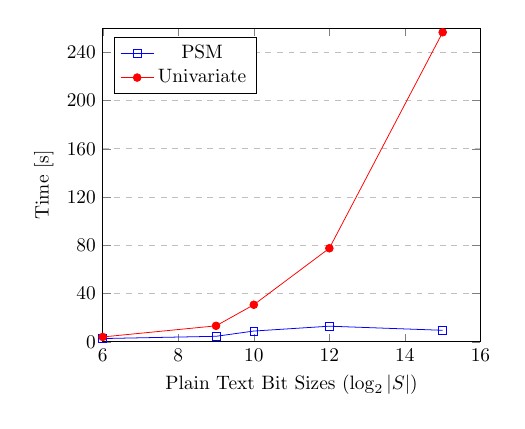
\begin{tikzpicture}[scale=0.70]
\begin{axis}[
    xlabel={Plain Text Bit Sizes ($\log_2{|S|}$)},
    ylabel={Time [s]},
    xmin=6, xmax=16,
    ymin=0, ymax=260,
    xtick={2,4,6,8,10,12,14,16},
    ytick={0,40,80,120,160,200,240},
    legend pos=north west,
    ymajorgrids=true,
    grid style=dashed,
]

\addplot[
    color=blue,
    mark=square,
    ]
    coordinates {
        (6,2.74577)(9,4.6201)(10,8.97098)(12,12.9959)(15,9.59417)
    };

\addplot[
    color=red,
    mark=*,
    ]
    coordinates {
    (6,4.07774)(9,13.2915)(10,30.7507)(12,77.5586)(15,256.502)
    };
    
\legend{PSM , Univariate}
    
\end{axis}
\end{tikzpicture}
\caption{Efficiency of Integer Comparison.}
\label{fig:integer}
\end{subfigure}
\begin{subfigure}{.33\textwidth}
\centering
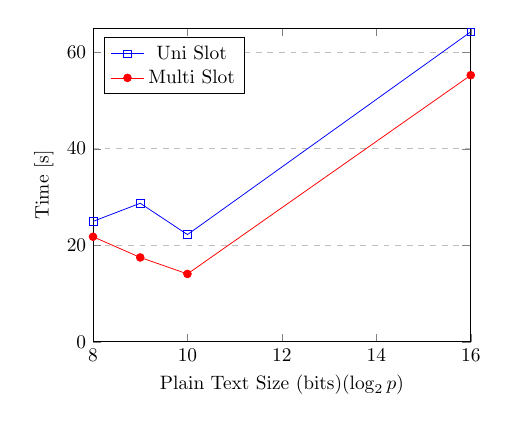
\begin{tikzpicture}[scale=0.7]
\begin{axis}[
    xlabel={Plain Text Size (bits)($\log_2{p}$)},
    ylabel={Time [s]},
    xmin=8, xmax=16,
    ymin=0, ymax=65,
    xtick={2,4,6,8,10,12,14,16},
    ytick={0,20,40,60},
    legend pos=north west,
    ymajorgrids=true,
    grid style=dashed,
]

\addplot[
    color=blue,
    mark=square,
    ]
    coordinates {
        (8,24.954)(9,28.7115)(10,22.2222)(16,64.215)
    };

\addplot[
    color=red,
    mark=*,
    ]
    coordinates {
    (8,21.7776)(9,17.4891)(10,14.0714)(16,55.2358)
    };
\legend{Uni Slot, Multi Slot}
    
\end{axis}
\end{tikzpicture}
\caption{PSM efficiency with plaintext size.}
\label{fig:string}
\end{subfigure}
\begin{subfigure}{.33\textwidth}
\centering
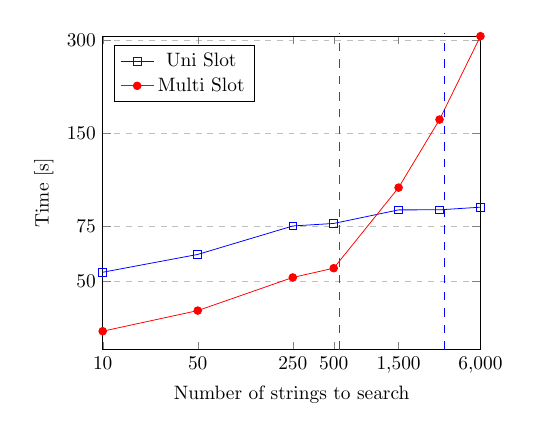
\begin{tikzpicture}[scale=0.7]
\begin{loglogaxis}[
    xlabel={Number of strings to search},
    ylabel={Time [s]},
    xmin=10, xmax=6000,
    ymin=30, ymax=310,
    log ticks with fixed point,
    xtick={10,50,250,500,1500,6000},
    ytick={50,75,150,300},
    legend pos=north west,
    ymajorgrids=true,
    grid style=dashed,
]

\addplot[
    color=blue,
    mark=square,
    ]
    coordinates {
        (10,53.42)(50,61)(250,75.4)(500,76.81)(1500,84.97)(3000,85)(6000,86.69)
    };

\addplot[
    color=red,
    mark=*,
    ]
    coordinates {
    (10,34.45)(50,40.16)(250,51.39)(500,55.06)(1500,100.29)(3000,166.41)(6000,309.51)
    };

\legend{Uni Slot, Multi Slot}
    
\end{loglogaxis}
\draw [red,dashed] (4.3,0) -- (4.3,5.75);
\draw [blue,dashed] (6.2,0) -- (6.2,5.75);
\end{tikzpicture}
\caption{PSM efficiency with set size.}
\label{fig:searchspace}
\end{subfigure}
\caption{PSM efficiency}
\end{figure*}

\subsubsection{String Comparison}
$\PSM$ handles string comparison in two ways, resulting from different packaging strategies. Both strategies require minor changes to the $\PSM$ algorithm. The first strategy, called MultiSlot, is to pack each string of size $e$ over $e$ plaintext slots, thus setting the number of strings encoded in each plaintext at most $b=\floor{l_{\Phi}/e}$. The second strategy, dubbed UniSlot, is more compact, but slightly less efficient. It takes advantage of the plaintext ring structure $\F_{p^{\delta}}$, where $\delta$ is the order of $p$ modulo $m$. When $\delta>1$, it is possible to pack several characters in a single slot.

The first strategy requires changing the function {\sc SumAll} because the slots containing the result of the slot-wise comparison of the string with each copy of the pattern must first be multiplied by each other and then only added together, thus requiring additional $\log_2{e}$ multiplications. The second strategy requires changing the {\sc IsZero} function to implement Fermat's Little Theorem on extension fields.
\begin{equation}\label{eq:iszero+}
    \mathrm{IsZero}(a) = 1 - a^{p^{\delta-1}} \bmod p
\end{equation}
Kim et al. \cite{kimEfficiencyFHEbasedPrivate2016} showed that this equation could be implemented with a multiplicative depth of $\ceil{\log_2{\delta}}+\ceil{\log_2{p-1}}$ by taking advantage of the homomorphic Frobenius automorphism $x \mapsto x^{p}$. Therefore, when $\delta=e$, the multiplicative depth of both methods is equal. However, this second strategy also requires $\delta-2$ automorphisms that do not consume depth but do consume time.

Both alternatives impose limits on the search space. The UniSlot strategy forces the size of the pattern string to be no larger than $p^{\delta}$ bits, while the MultiSlot strategy imposes a soft limit on the search space $|S|$. The limit of the UniSlot strategy may be eliminated by combining both strategies, thus packing each string in $e.\delta$ slots. To eliminate the limit of the MultiSlot strategy, the {\sc SubProd} call in Alg. \ref{alg:psm}, must be replaced by a call to a more complex {\sc SubMapAdd} function (Appendix \ref{app:psmalgorithms}).


Tab. \ref{tab:string} compares both strategies for different plaintext modulus $p$. The maximum string size $\nu$ in bytes is set to $\nu=d.\floor{\log_2{p}}/8$ for the UniSlot strategy and $\nu=e.\floor{\log_2{p}}/8$, with $e=16$, for the MultiSlot strategy. The biggest difference between the two approaches is the number of strings that may be compared simultaneously. The UniSlot strategy can, on average, compare ten times more strings simultaneously ($ss_{max}$). 

Regarding efficiency, the UniSlot version is slightly less efficient (Fig. \ref{fig:string}) due to additional $d-2$ automorphisms.

\begin{table}[htbp]
\setlength\tabcolsep{3pt}
\caption{String Equality Settings}
\begin{center}
\begin{tabular}{ccccccccc}
\hline
\multirow{2}{1em}{p} &  \multirow{2}{1em}{$\lambda$} &  \multicolumn{3}{c}{UniSlot} & & \multicolumn{3}{c}{MultiSlot} \\ \cline{3-5} \cline{7-9}
&& $\nu$ & $ss$ & T(s) & & $\nu$ & $ss$ & T(s) \\ \hline
257 &  163 &  21 & 1448 & 24.95 & & 16 & 90 & 21.78\\
521 &  141$^{\mathrm{a}}$&  24 & 1560 & 28.71 & & 18 & 159 & 17.49 \\
1031 &  133 &  21 & 1904 & 22.22 & & 20 & 119 & 14.07 \\
65537 &  164$^{\mathrm{b}}$ &  36 & 3480 & 64.22 & & 32 & 504 & 55.24 \\
\hline
\multicolumn{9}{l}{$^\mathrm{a,b}$ differ slightly in MultiSlot version: $^{\mathrm{a}}$135, $^{\mathrm{b}}$122.}
\end{tabular}
\label{tab:string}
\end{center}
\end{table}


\begin{comment}
\begin{figure}[htbp]

\centering
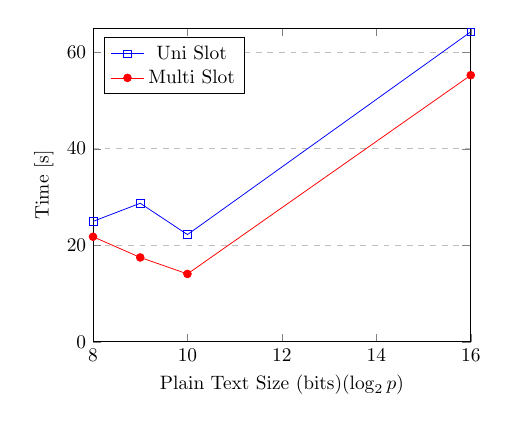
\begin{tikzpicture}[scale=0.7]
\begin{axis}[
    xlabel={Plain Text Size (bits)($\log_2{p}$)},
    ylabel={Time [s]},
    xmin=8, xmax=16,
    ymin=0, ymax=65,
    xtick={2,4,6,8,10,12,14,16},
    ytick={0,20,40,60},
    legend pos=north west,
    ymajorgrids=true,
    grid style=dashed,
]

\addplot[
    color=blue,
    mark=square,
    ]
    coordinates {
        (8,24.954)(9,28.7115)(10,22.2222)(16,64.215)
    };

\addplot[
    color=red,
    mark=*,
    ]
    coordinates {
    (8,21.7776)(9,17.4891)(10,14.0714)(16,55.2358)
    };
\legend{Uni Slot, Multi Slot}
    
\end{axis}
\end{tikzpicture}
\caption{PSM efficiency with plaintext size.}
\label{fig:string}
\end{figure}
\end{comment}

However, if the search space $|S|>ss_{max}$, then {\sc MultiSlot} is much less efficient due to the {\sc SubMapAdd} algorithm. Fig. \ref{fig:searchspace} depicts the time required to search for different set sizes $|S|$, for 16 character UTF-16 strings (last line of Tab. \ref{tab:string}). Notice that the slope of the {\sc MultiSlot} curve increases when the set to search is larger than $ss_{max}=504$, but that does not happen with {\sc UniSlot} when the search set is larger than $ss_{max}=3480$.

\begin{comment}
\begin{figure}[htbp]
\centering
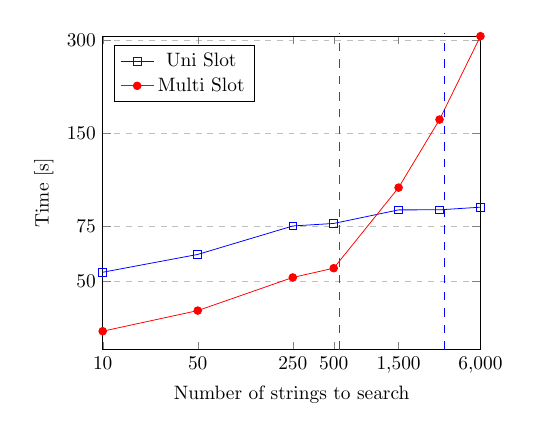
\begin{tikzpicture}[scale=0.7]
\begin{loglogaxis}[
    xlabel={Number of strings to search},
    ylabel={Time [s]},
    xmin=10, xmax=6000,
    ymin=30, ymax=310,
    log ticks with fixed point,
    xtick={10,50,250,500,1500,6000},
    ytick={50,75,150,300},
    legend pos=north west,
    ymajorgrids=true,
    grid style=dashed,
]

\addplot[
    color=blue,
    mark=square,
    ]
    coordinates {
        (10,53.42)(50,61)(250,75.4)(500,76.81)(1500,84.97)(3000,85)(6000,86.69)
    };

\addplot[
    color=red,
    mark=*,
    ]
    coordinates {
    (10,34.45)(50,40.16)(250,51.39)(500,55.06)(1500,100.29)(3000,166.41)(6000,309.51)
    };

\legend{Uni Slot, Multi Slot}
    
\end{loglogaxis}
\draw [red,dashed] (4.3,0) -- (4.3,5.75);
\draw [blue,dashed] (6.2,0) -- (6.2,5.75);
\end{tikzpicture}
\caption{MultiSlot vs UniSlot PSM efficiency with set size.}
\label{fig:searchspace}
\end{figure}
\end{comment}